\documentclass[lettersize, noapacite, twoside, HRI]{apa_HRI}


%\usepackage[utf8x]{inputenc}
\usepackage{times}

\usepackage{graphicx} 
\usepackage{subfigure}
\usepackage{paralist}

\usepackage{hyperref}

\usepackage{amsfonts}
\usepackage{mathtools}
\usepackage{url}
\usepackage{xspace}
\usepackage{booktabs}

\usepackage[natbibapa]{apacite}

\usepackage{tikz}
\usetikzlibrary{shapes,positioning,calc,decorations.pathreplacing}
\newcommand{\tikzmark}[1]{\tikz[overlay,remember picture] \node (#1) {};}

\usepackage[draft,nomargin,footnote]{fixme}

\graphicspath{{figs/}}

\newcommand{\eg}{\textit{e.g.}\xspace}
\newcommand{\etal}{\textit{et al.}\xspace}
\newcommand{\ie}{\textit{i.e.}\xspace}
\newcommand{\etc}{\textit{etc.}\xspace}
\newcommand{\vs}{\textit{vs.}\xspace}

\newcommand{\h}[1]{\textbf{H#1}\xspace}

\newcommand{\anti}{{$\mathcal{A}_{start}$\xspace}}
\newcommand{\antf}{{$\mathcal{A}_{end}$\xspace}}
\newcommand{\deltaant}{{$\Delta_{\mathcal{A}}$\xspace}}


\rightheader{Gazing at the Robot's Head Reflects our Tendency to Anthropomorphise}   % This should be the title, or a shortened version of the title if your title is long.
\leftheader{Lemaignan et al.}	  % For one or two authors, include both authors last names.  For three or more, use first author's last name et al.
\title{Gazing at the Robot's Head Reflects our Tendency to Anthropomorphise}

\author{S\'everin Lemaignan, Kshitij Sharma, Ashish Ranjan Jha, Pierre
Dillenbourg}
\affiliation{CHILI Lab, \'Ecole Polytechnique F\'ed\'erale de Lausanne}

\acknowledgements{\url{firstname.lastname@epfl.ch}}

\abstract{

Could the way we look at robots betray our anthropomorphic ascriptions to the
machine? We show in the article that indeed, the duration of gaze fixations on
the head of a humanoid robot reflects one's tendency to anthropomorphise the
robot.  We reach this conclusion by building on an novel experimental protocol
involving cognitive priming: participants are shown a set of stimuli that are
visually identical and yet induce different assumptions regarding the cognitive
capabilities of the robot. By correlating the resulting gaze patterns with
answers to established questionnaires on anthropomorphic attributions, we show
that fixations on the head of the robot reflect how we anthropomorphize the
machine. Besides, by comparing this gazing behaviour to a human baseline, we further
show that people with a generally higher tendency to anthropomorphise exhibit
similar gaze patterns when they look either at humans or robots.

}

\keywords{human-robot interaction, anthropomorphism, cognitive priming, eye-tracking, gaze patterns}

\begin{document}
\maketitle

\section{Introduction}

Researchers in robotics often tend to see anthropomorphism as the static set of
human-like features of a robot (like its shape, its speech capabilities, facial
expressions, etc.). Following~\citet{fink_anthropomorphism_2012}, we refer to
these characteristics as the \emph{anthropomorphic design} of the robot, and we
call instead \emph{anthropomorphism} the \emph{social phenomenon} that arises
from the (real or imagined) interaction between a non-human agent (a robot in
our case) and a human~\citep{persson_anthropomorphism_2000}. As such,
anthropomorphism includes the perception of emotional states, motivations,
intentions in the non-human agent, and, conversely, the ascriptions of those
qualities to them~\citep{epley_when_2008}.

Being a rich, compound trait that characterises the bonds between humans
and robots, the field of human-robot interaction (HRI) has long
attempted to assess and manipulate the anthropomorphic attributes we ascribe to robots.
While modifying the anthropomorphic \emph{design} of robots is conceptually
easy, influencing the underlying psychological phenomenon is less
obvious, although possibly as effective.

One way consists in manipulating the context of use of the robot: when social,
entertaining or playful, it elicits more anthropomorphic attributions compared
routine or focused, serious situations (security, rescue, \etc).
\citet{joosse_what_2013} showed for instance that users would ascribe
different personalities to the same robot (a {\sc nao} humanoid) when it was
used in a different task context (cleaning task \vs tour guide). Along the same
line, \citet{goetz_cooperation_2002} found that people prefer a serious robot
for serious tasks and a less serious robot for more playful tasks. Also related,
\citet{kaplan_free_2000} discussed how the uselessness of the robot impacts our
tendency to anthropomorphise it: artificial pets like AIBO have no real purpose,
in a sense that they do not provide any kind of service, and this very aspect
increases people's tendency to anthropomorphise them.

We may hypothesise that these results are a consequence of different
expectations we form about the robot depending on the context: when a machine is
embedded in a social situation, we expect it to exhibit certain
social skills. The experiments found so far in the literature contrast prototypical
\emph{opposite} interaction situations (routine \vs playful, typically boring \vs typically
intellectual): while they do confirm that the interaction context impacts our
perception of the robot, the stark contrast of the conditions makes it difficult
to finely analyse the psychological determinants that explain the different
perception of the robot. This is made worst by the common reliance on
questionnaires to measure anthropomorphism, with the associated issue of
post-hoc reconstruction (we elaborate on this hereafter).

This article introduces a different experimental design and a novel methodology
to measure \emph{in-the-moment} anthropomorphic attributions.  Our approach is
built on a combination of cognitive priming and eye-tracking. By doing so, we
evidence specific gaze fixations on the head of the robot when the participants
are primed with higher expectations regarding the cognitive skills of the robot.
We then show how subtle interaction manipulations do significantly impact our
tendency to ascribe human traits to machines, to eventually establish the link
between head fixations and anthropomorphic ascriptions.

\subsection{Measuring Anthropomorphism}

Assessing anthropomorphic attributions during a human-robot interaction is an
indirect mean to explore the intricate -- and dynamic -- bonds that build up
between the robot and its human partner. As such, a lot of literature in HRI has
investigated means of measuring anthropomorphism. This indeed raises 
methodological challenges, due to high inter-personal variations in
one's tendency to anthropomorphise, and the dynamic nature of
anthropomorphic attributions~\citep{lemaignan2014dynamics}.

One phenomenon requires particular attention: well established in the
psychological literature in terms of \emph{impulsive} or \emph{automatic} \vs
\emph{reflective} behaviours~\citep{strack2004reflective}, the way we behave and
perceive \emph{in-the-moment} is significantly different from what results from
a thoughtful (and slower) reflection on the situation. As noted by
\citet{takayama_perspectives_2012} for instance, this also impacts our
perspective on agency, and in fact, as shown by~\citet{nass_machines_2000}, in
the first phase of interaction with a robot, people might respond mindlessly,
and only after the so-called \emph{familiarisation} period, one might respond in
a more conscious, reflective manner. The typical illustration of this mechanism
is found in~\citet{reeves_media_1996} who showed that participants who would
interact with technologies in ways similar to how they interact with people,
would however {\it a posteriori} typically deny having performed an human-like
interaction.

Yet, most of the methodologies available to assess anthropomorphic ascriptions
in HRI are limited to post-interaction measurement, mainly in the form of closed
questionnaires or rating scales. The Godspeed
questionnaire~\citep{bartneck_measurement_2008}, and in particular, its subpart
focused on anthropomorphism, is the main validated questionnaire to assess
anthropomorphism. On 5-point semantic differential scales, people are asked to
rate the following constructs: fake \vs natural, machinelike \vs humanlike,
unconscious \vs conscious, artificial \vs lifelike, moving rigidly \vs moving
elegantly. Because the concept of ``human-likeness'' itself is complex and
abstract, \citet{kahn_jr._robotic_2006} suggest to ask for more concrete
constructs that are typical or unique of the concept of ``human-likeness'', and
\citet{ruijten_introducing_2014} propose for instance a 25-items questionnaire to
measure various concrete aspects of human-likeness. Other
researchers~\citep{zlotowski2014dimensions,salem2015would} also applied a
two-dimensional scale measuring \emph{Human Nature} and \emph{Uniquely Human}
traits of robots, based on an original proposal by
\citet{haslam2008attributing}.

We explore hereafter a different approach to measure anthropomorphism, based on
eye-tracking. By looking at the eyes fixation on the head of the robot, we show
significantly different gazing behaviours in two experimental conditions that
differ in terms of the (projected) robot's human-likeness. This eye-tracking
based metric is behavioural -- hence not prone to post-hoc reconstruction by the
participants -- and \emph{in-the-moment} -- mitigating the impact of a reflective
elaboration on the nature of the human-robot interaction. We believe that these
two improvements over existing techniques provide a solid ground for the study
of the socio-cognitive bonds that establish between humans and robots when they
interact.

\subsection{Cognitive Priming and Interaction Situation}
\label{cognitive-priming}

Cognitive priming is the primary mean of condition manipulation that we rely on.
Many previous studies have investigated how cognitive and/or affective priming
influence human perception of an input stimulus. \cite{zajonc1980feeling}
advocated the use of affective priming and proposed that the affective reactions
can be elicited with minimal stimulated input: \cite{murphy1993affect} found in
a series of studies where participants were shown happy and angry faces as a
priming method, that the participants' perceptions of positive emotions were
higher and quicker when the priming was a happy face than for those who were
primed with a angry face. The gender of the priming faces, however had no effect
on the participants' perception.

\cite{forgas1987mood} showed that priming participants with positive or negative
moods affects their person-perception judgement\footnote{Person-perception
judgement is a task where the participants are asked to read a few
characteristics of an unknown person; and once they have read the description
the participants are then asked to provide their perception about the target
person}. In their study, they used a test with manipulated positive or negative
feedback to prime the mood of the participants in a positive or negative manner.
The results showed that the priming influenced their person-perception, \ie the
positively primed participants provided more positive remarks about a new,
unknown face, while the negatively primed participants made more negative
remarks. Moreover, the participants in both the priming conditions spent more
time elaborating on the specific characteristics they were primed with. This
shows that mood priming influenced not only the participants' perceptions, but
also their behaviours during the test.

Similarly, \cite{yi1990cognitive} used specific attributes of a car to prime
participants before they watched an advertisement about cars. The advertisement
discussed characteristics of imaginary cars in terms of their safety and fuel
efficiency.  The priming stimulus had manipulated the size of the car, as well
as the tone of the description. The results showed that both the tone (affective
priming) and the size (cognitive priming) affects the likeability of the car.
In the context of advertising, a number of studies suggest that the context
(cognitive priming) influences the perception of the advertisement by the
audience, and therefore, its effectiveness~\citep{singh1987arousal,soldow1981response}.

In an fMRI study with music notes, \cite{tillmann2006cognitive} showed that
different parts of the frontal cortex gets activated when the participants were
primed with sung or instrumental music. In their experiment, the participants were
asked to listen the first seven notes in either sung or instrumental manner
(cognitive priming) and then to identify the relation between the first seven
and the eighth note. The results showed that the participants showed a higher
activation in the inferior frontal cortex when primed with the sung notes than
when they were primed with the instrumental notes.

\cite{rholes1987emotional} showed that the memory recall is affected by the tone
(affective priming) of self-evaluation statement: In an experiment, where
the participants were given a set of positive or negative self-evaluation
statements before being asked to recall a few good and bad memories from their
past, the participants were faster in recalling good memories when they were
given a positive self-evaluation test and vice-versa.

All the above studies show that cognitive and/or affective priming can alter
both the perception by the participant of a target stimulus, and the behaviour
of the participant while processing the stimulus. Some of the studies also
evidenced interactions between cognitive and affective
priming~\citep{yi1990cognitive,storbeck2008affective}.

We focus here on cognitive priming: as~\cite{baldwin1990priming} pointed out, we
expect that cognitive priming may activate a relationship schema between the
priming stimulus (the context of the interaction) and the
target stimulus (the interaction situation, and in particular, the robot).
More specifically, we designed stimuli in which the way the robot is given
commands pre-supposes a specific interaction situation (more or less
`human-like') and is expected in turn to alter the way the participants perceive the
actions of the robot.

We use a neutral mood/tone (no affective priming) and, as detailed in the
Methodology section hereafter, two cognitive priming conditions (hereafter
referred as `machine-like' and `human-like').



\subsection{Hypotheses}

As suggested in the previous section, we aim at verifying the following research
hypothesis \h{}: the level of anthropomorphism ascribed by a human to a robot can be
effectively assessed by measuring the human's gaze fixations on the robot's head.

Our methodology involves showing participants video stimuli that elicit
different levels of anthropomorphism, and measuring gaze fixations over the
course of the video clips. To be suitable for an eye-tracking experiment, the
video stimuli must be visually identical between conditions, and therefore
we have to rely on non-visual cues to elicit different anthropomorphic
projections. We choose to use cognitive priming with audio cues, as detailed in
the next section.

This approach allows us to decompose the hypothesis \h{} into two simpler
hypotheses \h{1} and \h{2}: we want first to verify that cognitive priming
enables us to effectively manipulate the attribution of human-likeness to robots
(\h{1}).  We need next to verify that in the case of higher anthropomorphic
attributions, the participants' gaze will be directed significantly more towards
the head of the robot than in the case of low anthropomorphic attributions
(\h{2}).

If verified, these hypotheses would allow us to conclude that in a given
human-robot interaction situation, gaze fixations on a robot's head reflects the
ascription of anthropomorphic features to the robot. This would suggest that a
relatively simple biometric and in-the-moment measure (eye-tracking) can
effectively inform us about occurring anthropomorphic projections.


\vspace{1em}

Besides, our experimental design allows to examine two additional hypotheses:

\begin{itemize}
    \item people who generally tend to anthropomorphise exhibit gazing
        behaviours that are similar when looking either at humans or robots, and
        reciprocally (\h{3}). If this is verified, this would confirm that our
        gazing behaviour towards agents is impacted by our tendency to
        anthropomorphise.

    \item the mere observation of a robot acting in an \emph{human-like}
        situation suffice to increase the level of
        anthropomorphic attributions to robots \emph{in general} (\h{4}).
\end{itemize}

%If all these hypotheses are verified, the findings can be summarised as follow:
%\h{1} shows that our manipulation (based on cognitive priming) does effectively
%elicit lower or higher expectations in terms of the cognitive capabilities of
%the robot; \h{4} shows that these expectations influence our tendency to
%anthropomorphise robots in general; in parallel, \h{3} shows that these same expectations
%shape the way we look at the robot by eliciting specific eye fixations on the
%head of the robot; finally, \h{2} suggests that the fixation on the head
%reflects human-likeliness and supports the thesis that head fixation can be used
%as a behavioural measure of anthropomorphism.

%Figure~\ref{hyps} illustrate how these four hypotheses relate to \emph{a)}
%cognitive priming, \emph{b)} anthropomorphic attributions, and \emph{c)} gaze
%patterns.
%
%\begin{figure}[ht]
%\centering
%
%\resizebox{0.5\linewidth}{!}{%
%
%\begin{tikzpicture}[
%    >=latex,
%    every edge/.style={->,draw, very thick},
%    every node/.style={draw, circle, text centered, text width=2.7cm}]
%
%    \node at (0,0) (ctxt) {cognitive priming};
%    \node at (-3,-3) (anthro) {Anthropomorphic attributions};
%    \node at (3,-3)[circle split, text width=2.5cm] (gaze) {\textit{\small Fixations \\on head} \nodepart{lower} \textit{\small Gaze
%distribution \\differences}};
%    \node [draw=none,anchor=east,left=-0.5cm of gaze.west] (gazecap) {\large Gaze:};
%
%    \path[every node/.style={draw=none}]
%            (ctxt) edge [bend right] node[left] {\h{1}, \h{4}} (anthro)
%            (ctxt) edge [bend left] node[right] {\h{3}} (gaze.north)
%            (anthro) edge [bend right] node[above] {\h{2}} (gaze.south);
%\end{tikzpicture}
%}
%
%\caption{Hypotheses of interactions between the three main concepts studied in
%the article. Arrows mean ``A impacts B''.}
%
%    \label{hyps}
%\end{figure}


\section{Experimental Design}
\label{sec:design}

As mentioned, this study is built as an eye-tracking experiment (using a stationary
eye-tracker SMI RED 250) where participants watch short videos of an agent --
either a robot (the Aldebaran Robotics' Nao) or a human -- performing simple tasks
(picking an object or pointing toward a sound source) after being primed.  The
priming is designed to elicit either low cognitive ascriptions onto the robot
(leading to what we call hereafter a \emph{machine-like} interaction situation)
or richer cognitive ascriptions (leading to what we call a \emph{human-like}
interaction situation).

Besides eye-tracking, the participants' perception of robots is assessed through a
pre- and a post-questionnaire, described below.

\subsection{Conditions}

The study follows a 2$\times$2 design, summarised in figure~\ref{table:design}.
Our two independent variables are the level of cognitive priming (\emph{machine-like}
\vs \emph{human-like}) and the nature of the agent appearing in the stimulus (a robot
or a human).

The cognitive priming manipulation is established by having a speaker imply
different cognitive capacities in the robot.

\begin{figure}[ht!]
    \vspace{2em}
    \centering
    \small

    \tikzmark{top}

    \tikzmark{left}
    \begin{tabular}{l|p{4.3cm}|p{4.3cm}}
        & \tikzmark{top1} Machine-like cognitive priming & Human-like cognitive priming \tikzmark{top2}  \\
        \hline
        \tikzmark{left1} Robot & {\bf A}: \emph{``Pick the brown toy''} & {\bf A}: \emph{``Pick your favourite toy''} \\
                               & {\bf B}: \emph{``Point at the noise''} & {\bf B}: \emph{``Point at the crying baby''} \\
        \hline
        \tikzmark{left2} Human & {\bf A}: \emph{``Pick the brown toy''} & {\bf A}: \emph{``Pick your favourite toy''} \\ 
                               & {\bf B}: \emph{``Point at the noise''} & {\bf B}: \emph{``Point at the crying baby''}\tikzmark{bottom} \\
        \end{tabular}

    % draw the over- and side-braces
    \begin{tikzpicture}[overlay, remember picture]

        \draw [decoration={brace,amplitude=0.5em},decorate,thick]
        (top -| top1.west) --  (top -| bottom.east) node[midway, above=0.5em] {\scriptsize between subjects};

        \draw [decoration={brace,amplitude=0.5em},decorate,thick]
        ($(left |- bottom)+(1.4,-0.3)$) --  ($(left |- left1.north)+(1.4,0.2)$) node[midway,left=1em,rotate=90,anchor=south] {\scriptsize within subject};
    \end{tikzpicture}
    %%%

    \caption{\small The study follows a 2$\times$2 design: the \emph{robot} vs
        \emph{human} condition is within subject, while the \emph{machine-like
        cognitive priming} \vs \emph{human-like cognitive priming} is between subjects.
        Two stimuli (\emph{Picking} task {\bf A}, and \emph{Pointing} task
        {\bf B}) were shown to the participants, introduced by brief verbal
        commands, reproduced in the table. Figure~\ref{fig:stimuli} shows
        pictures of the four stimuli.}

    \label{table:design}
\end{figure}


\subsection{Video Stimuli}

Four different video stimuli were filmed (figure~\ref{fig:stimuli}, see appendix
for download link): two
different tasks (picking a stuffed animal, referred hereafter as the
\emph{Picking} task, and pointing towards a source of sound, referred as the
\emph{Pointing} task) acted either by a human or a robot. Video stimuli were
realised in studio conditions. All videos followed the same simple structure: an
initial audio command (spoken by an invisible person), followed by the task
being executed.

The human actor was instructed to follow as closely as possible the actions and
attitudes of the robot (left/right glances, hesitations, gestures), while keeping a
natural, \emph{human-like} general behaviour. As a result, the length of human videos
(57 seconds in total for the two tasks) was shorter than robot videos (110
seconds) due to the robot being usually slower in performing actions (in
particular walks) compared to human.\footnote{To make sure the difference of
video length does not bias gaze distributions, we ran a $\chi^2$ test between
the gaze distributions of the first half and the second half of the robot
videos: no significant difference was found ($\chi^2[DF=4]=.0066, p=1$).}

The audio (and audio only) of these four videos was then edited to create two
sets of stimuli: one for the \emph{machine-like cognitive priming} condition, one for
the \emph{human-like cognitive priming} condition. The audio editing consisted of 
inserting different commands to initiate the tasks (reported in
figure~\ref{table:design}): in the \emph{Picking} task for instance, the object
that the agent had to pick was described either as a \emph{``brown toy''} or as
\emph{``your favourite toy''}. In the former case, the object was referred through
visible, objective features. They do not presuppose as complex cognitive capabilities
as in the latter case where the priming is expected to elicit the assumption
that the robot has tastes and preferences such as it can choose a toy as its favourite.

This simple verbal prompt (\emph{``brown toy''} \vs \emph{``your favourite
toy''}) creates a set of expectations regarding the cognitive capabilities of
the robot and leads to a different perceptions of the interaction situation (the
task performed by the robot is seen by the participant as more
\emph{machine-like} or more \emph{human-like}). We reinforced this effect in the
\emph{Pointing} task: not only the verbal prompt (\emph{``point at the noise''}
\vs \emph{``point at the crying baby''}) but also the background sound played by
the speakers during the task was altered: either a repetitive beep
(\emph{machine-like} situation) or the sound of a crying baby (\emph{human-like}
situation).

\begin{figure}
    \centering
    \subfigure[\emph{Picking} task, robot condition]{
        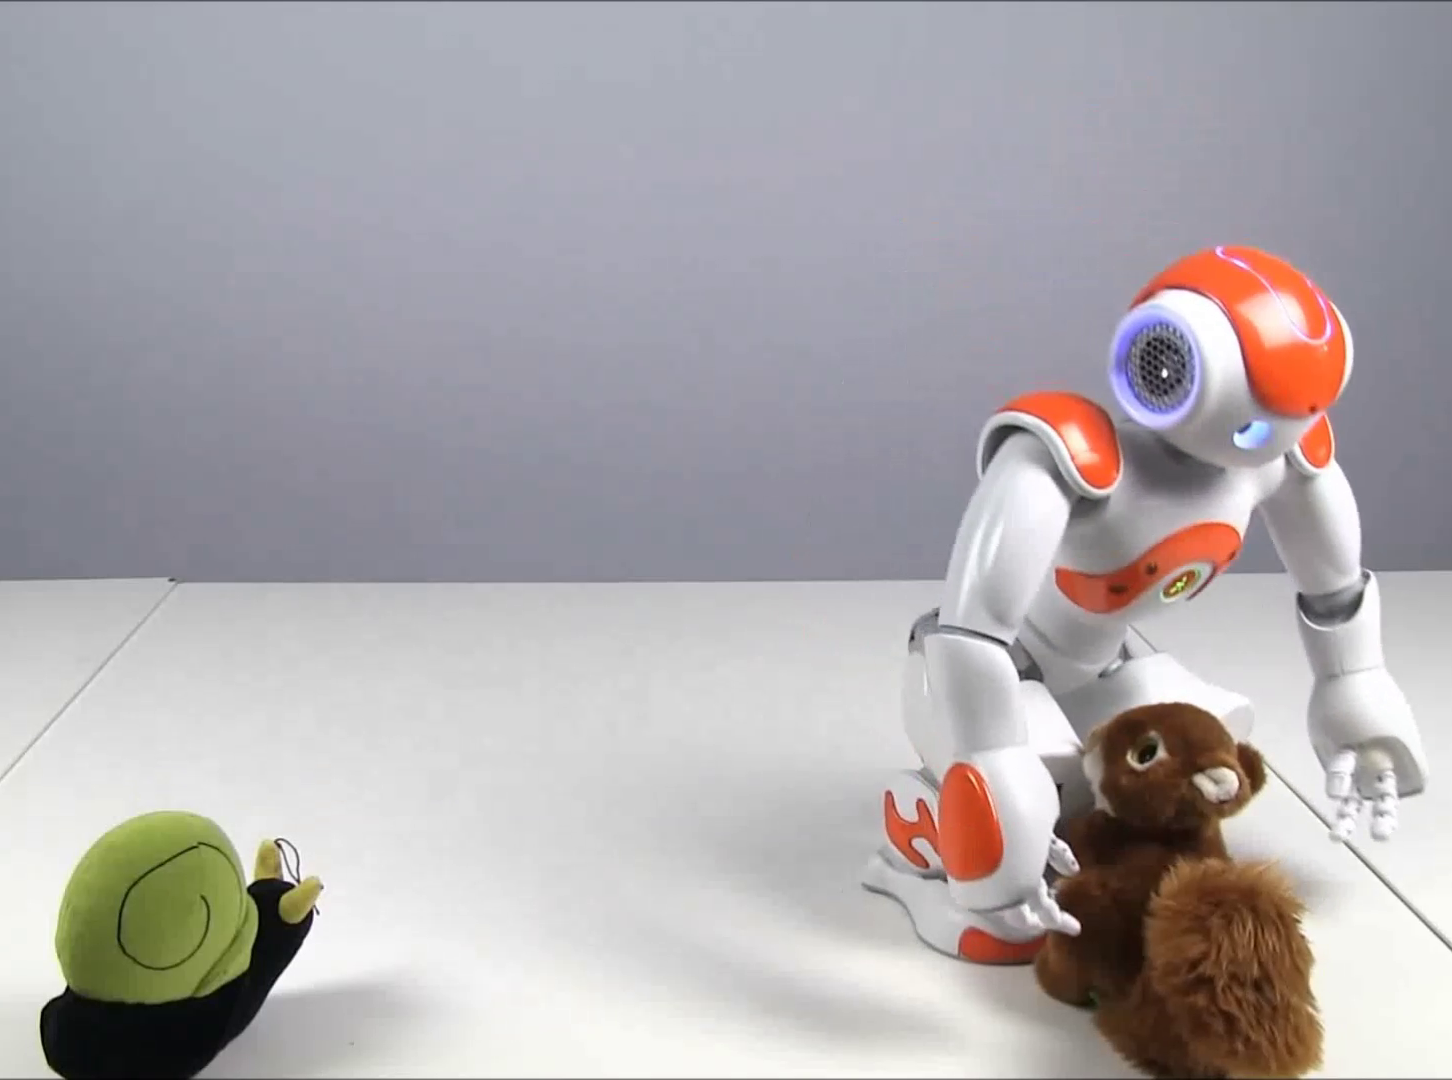
\includegraphics[height=5cm]{stimulus-robot-toys}
    }
    \subfigure[\emph{Picking} task, human condition]{
        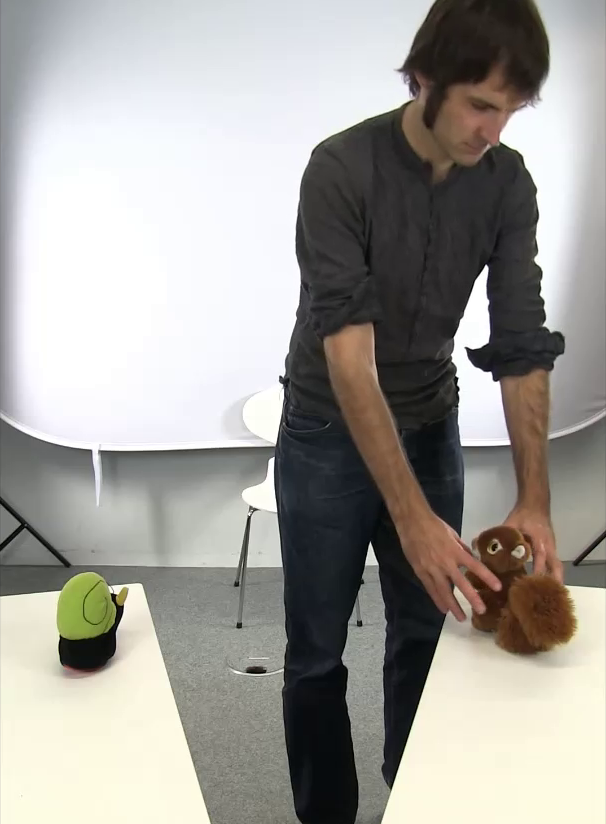
\includegraphics[height=5cm]{stimulus-human-toys}
    }

    \subfigure[\emph{Pointing} task, robot condition]{
        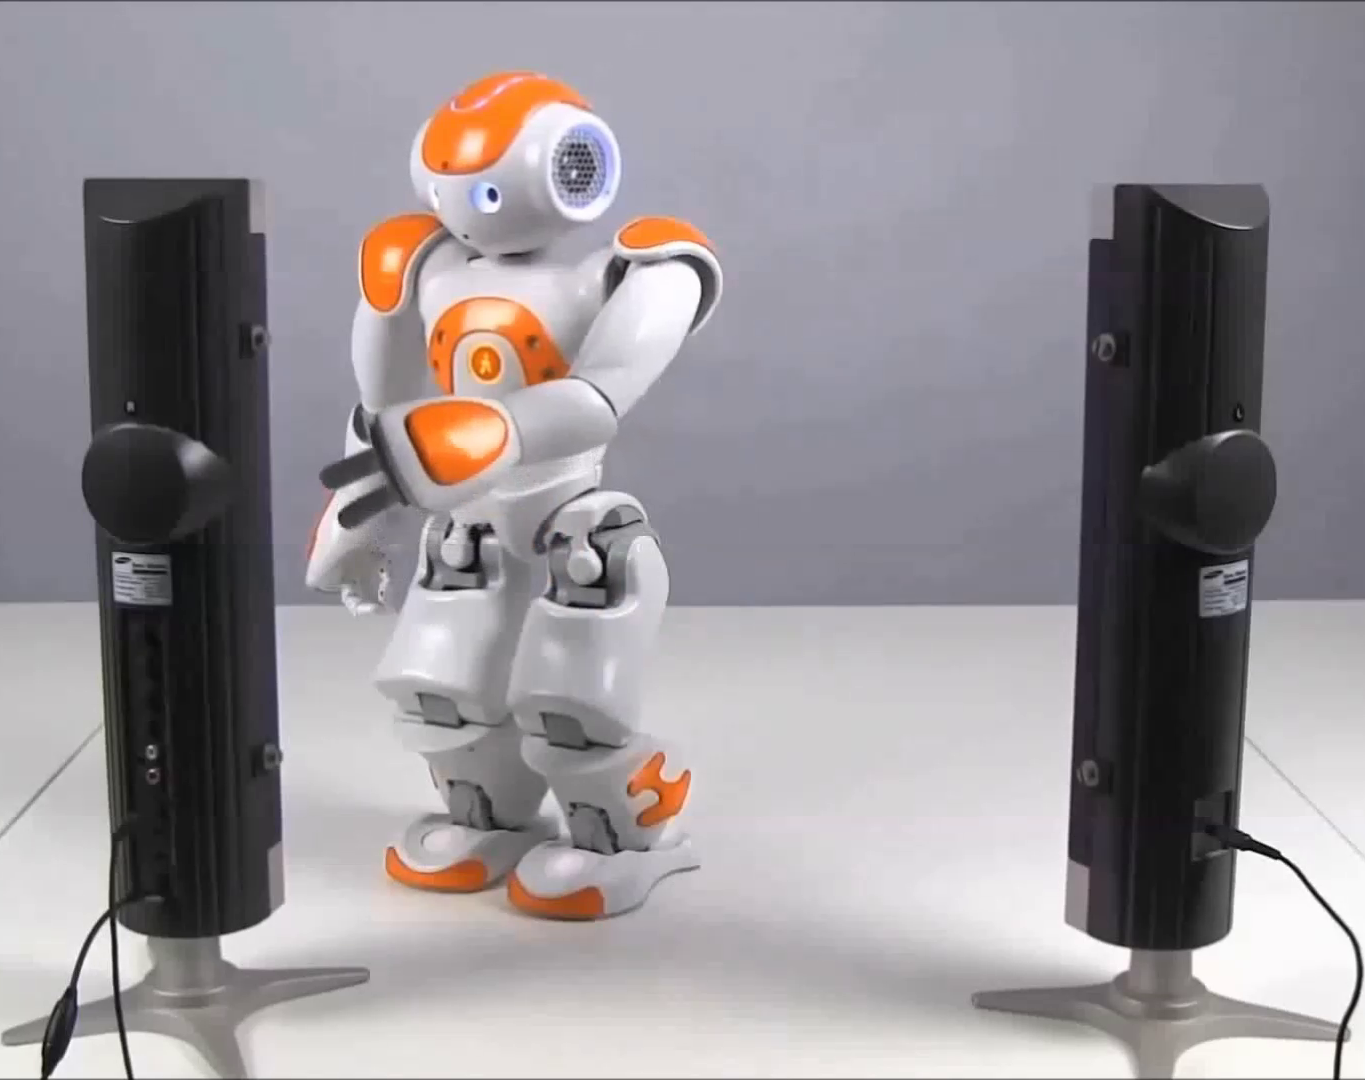
\includegraphics[height=5cm]{stimulus-robot-noise}
    }
    \subfigure[\emph{Pointing} task, human condition]{
        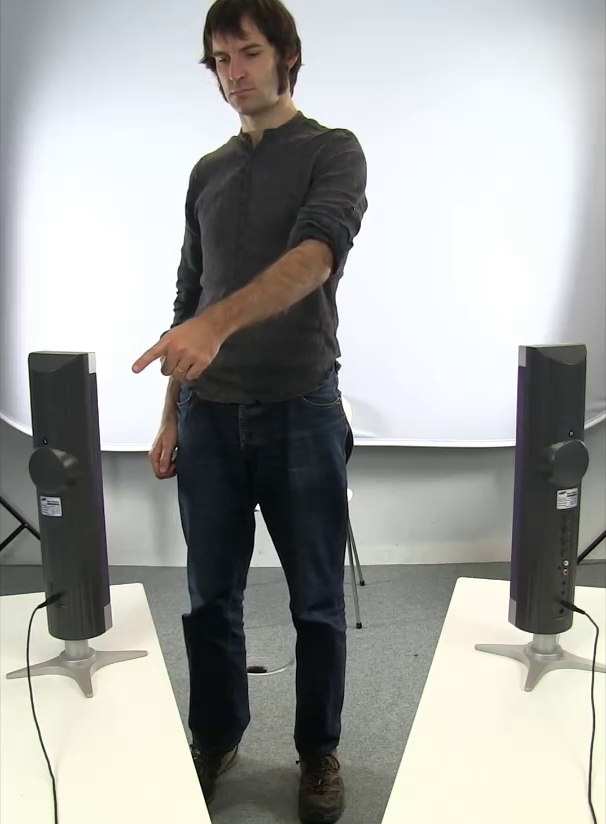
\includegraphics[height=5cm]{stimulus-human-noise}
    }


    \caption{\small Screenshots of the 2$\times$2 stimuli. Note that the images above have been
    slightly cropped: the original video are framed so that the agent (robot or
    human) always remains entirely visible.}
    \label{fig:stimuli}
\end{figure}

Section~\ref{stimuli_design}, at the end of the article, specifically discusses
the design constraints that were accounted for while creating the above stimuli.

\subsection{Questionnaires}

Before starting the experiment, the participants were asked to fill a
pre-questionnaire (available in appendix) which had 49 questions (5-point Likert scale). The
questionnaire included questions assessing their familiarity with robots, 10
items from the \emph{Big-Five} personality questionnaire, 15 questions taken from
Godspeed questionnaire (questions related to \emph{anthropomorphism},
\emph{likeability} and \emph{perceived intelligence}) and 20 questions rating
human-likeness of robots (from~\cite{ruijten_introducing_2014}). The pre-questionnaire
typically took 5 minutes for participants to complete. A subset of the results was turned into
a score noted \anti{} (\emph{initial tendency to anthropomorphise}) following a
method presented below (section~\ref{questionnaires_processing}).

The post-questionnaire (available in appendix) was administered at the end of the experiment, and was
identical to the pre-questionnaire, except that the personality questions were omitted and a
manipulation check question was added (\emph{``In your opinion, the tasks that
you watched were more: A robot kind of task ... A human kind of task''}, on a 5
point scale -- the phrasing was chosen over more the direct ``Machine-like'' \vs
``Human-like'' to mitigate the impact of a possible reflective moral judgement
on human-likeness).
This questionnaire typically took 3 to 4 minutes to complete. The resulting score is
noted \antf{} (\emph{final tendency to anthropomorphism}).

\anti{}, \antf{} and the difference \deltaant measured for each participant between
the pre- and post-questionnaires form the dependent variables of our experiment.
\deltaant, in particular, reflects the impact of the video stimuli on the
anthropomorphic perception that they have of robots \emph{in general}: the
Godspeed questions used in the questionnaires are not specific to the Nao robot
used in this particular experiment, and indeed assess how humans perceive robots
in a broad sense.

\section{Method}


%Figure~\ref{course_of_study} gives an overview of the protocol, detailed
%hereafter.
%
%\begin{figure}[ht]
%\centering
%
%\begin{tikzpicture}[
%    >=latex,
%    every edge/.style={<-,draw, very thick},
%    every node/.style={draw, text centered, text width=5cm}]
%
%    \node (n1) at (0,0) {Consent form};
%    \node (n2) [below=of n1] {Familiarization}
%        edge (n1);
%    \node (n3) [below=of n2] {Pre-questionnaire}
%        edge (n2);
%    \node (n4) [below=of n3] {Videos}
%        edge (n3);
%    \node (n5) [below=of n4] {Post-questionnaire}
%        edge (n4);
%
%\end{tikzpicture}
%    \caption{Overview of the course of the study}
%    \label{course_of_study}
%\end{figure}

\subsection{Participants}

We ran the study with 56 participants ($M = 20.9$ years old, $SD = 3.9$, 31 females and
25 males).  The participants were recruited amongst students of our university.
To avoid students with a high familiarity with robots and artificial intelligent
systems, Computer Science and Electronics students were excluded. This was
\textit{a posteriori} confirmed by the questionnaire responses: no participants
reported as being very familiar with robots, 8 reported some familiarity
and 7 out of 56 owned a domestic robot (vacuum cleaner).

As stated previously, the study followed a 2$\times$2 design
(table~\ref{table:design}): the \emph{machine-like} \vs \emph{human-like
cognitive priming} condition was between-subjects. 30 participants performed the
\emph{human-like cognitive} tasks while 26 were in the \emph{machine-like
cognitive} condition. The \emph{robot} \vs \emph{human} condition was
within-subject. The study lasted in average 15 minutes per participant.

\subsection{Procedure}

\subsubsection{Familiarisation and Pre-questionnaire}

Before starting the experiment, participants were made to read, understand and sign a
consent form. Participants were then asked to fill the 49 questions of
the pre-questionnaire, with a 10 minutes time limit (that none of the participants
reached).

After the pre-questionnaire, we invited the participants to an initial
free interaction with a powered-off Nao robot (we did not constraint
the time, and participants played between 2 and 3 minutes with the robot).
The purpose of this pre-interaction was to get the participants acquainted with the
robot appearance, shape and range of motions it could possibly perform, so as to
mitigate the (visual) novelty of the robot that would lead to possible
gaze artifacts (for instance, gaze fixations on salient peculiarities of the
robot, like the visible gears, or gaze exploration of the robot's body when the robot
starts to move).

\subsubsection{Stimuli Screening}

We then presented the stationary eye-tracker, conducted a brief eye-tracker
calibration procedure (all participants could be successfully tracked), and the
participants' gaze was recorded while they watched the \emph{robot} and
\emph{human} interaction stimuli. The order of stimulus presentation
was counter-balanced over the participants.

\subsubsection{Post-questionnaire and Conclusion}

Finally, the participants were asked to fill a post-questionnaire.
Before leaving, possible questions on the purpose of the study were
answered and each participant was given a compensation equivalent to EUR 10.

\subsection{Measures}

\subsubsection{Gaze Variables}

As seen in figure~\ref{fig:aoi}, we defined 10 Areas of Interest (AOIs): one on
the head of the agent (robot or human), two on the arms (left and right), two on
the hands, two on the legs and one on the torso. Besides, we defined one area of
interest per toy or speaker (depending on the stimulus).

\begin{figure}
    \centering
    \subfigure[\emph{Picking} task, robot condition]
    {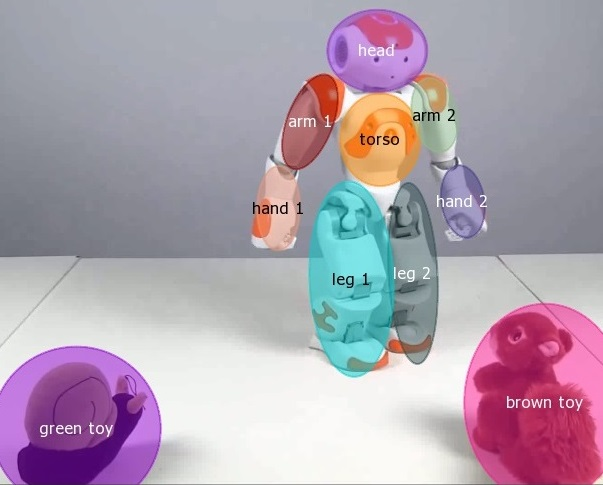
\includegraphics[height=5cm]{aoi-robot}\label{fig:aoi-toys}}
    \subfigure[\emph{Pointing} task, human condition]
    {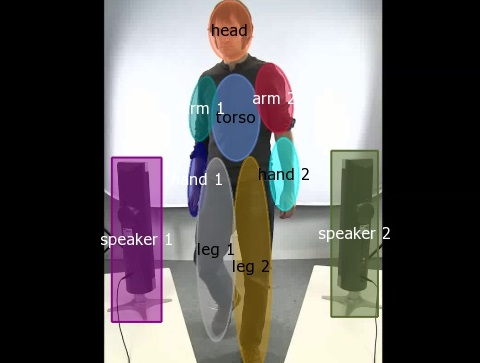
\includegraphics[height=5cm]{aoi-human}\label{fig:aoi-noise}}

    \caption{Areas of Interest (AOIs) used for the gaze analysis}
    \label{fig:aoi}
\end{figure}

We recorded the fixations on each of these zones and normalised them by
the full duration of the video stimuli and the surface of AOIs between the robot
and human conditions. We finally analysed their distribution, producing what we call \emph{gaze
patterns}.

To compare gazing behaviours across the robot and human conditions, we besides
computed a \emph{gaze distribution difference} over the 10 AOIs ($N=10$):

{\Large
\[
    \delta_{\mathcal{H}, \mathcal{R}}^{\text{gaze}} =
    \frac{\sum\limits_{{\text{{\sc aoi}s}}}\left |
    \frac{\text{Duration}_{\text{Human}}^{\text{\sc
aoi}}}{\text{Area}_{\text{Human}}^{\text{\sc aoi}}} -
\frac{\text{Duration}_{\text{Robot}}^{\text{\sc
aoi}}}{\text{Area}_{\text{Robot}}^{\text{\sc aoi}}} \right |}{N}
\]
}

TBD: editor comment here is correct: "a non-difference can come about as a
result of many counterveiling differences". He suggests instead "head-to-rest"
(or "head-to-[arm+hand]") difference for robot vs human

%As the lengths of the human's stimuli are different from the robot's ones, and
%the visual surface of the human body larger than the robot's, both \emph{Time}
%and \emph{Area} are normalised, respectively for the video length and the total
%area of the AOIs.

\subsubsection{Questionnaires Processing}
\label{questionnaires_processing}

Questionnaires were coded and two values, the \emph{initial tendency to
anthropomorphise} \anti{} and the \emph{final tendency to anthropomorphise} \antf{}
were computed, respectively from the pre- and post-questionnaires.

These values were computed by a direct sum of the rating provided by the
participants for the Godspeed's questions in the categories
\emph{anthropomorphism} and \emph{likeability}. These ten questions were rated
between -2 and 2, hence \anti{} and \antf{} vary between -20 and 20. The other
questions were not used for this study.

TBD: why anthropomorphism and likeability scales?

\section{Results}

Based on the experiments conducted on 56 participants in the human and robot
interactions across \emph{machine-like} and \emph{human-like cognitive priming} conditions,
we have the following results.\footnote{The detailed statistics and code used
    for obtaining the results are available here :
\url{https://github.com/chili-epfl/anthropomorphism-eyetracking}.}

%\subsection{General Biases}
First of all, we checked if there were any direct effects of the age, gender,
familiarity with robot and robot ownership of the participants on the different
aforementioned variables. We did not observe any such significant effects. 


%While testing for all the 4 hypotheses, we observed no significant bias with
%respect to age, gender, familiarity with robot and robot ownership
%of the participants, \ie there was no effects to be found between these factors
%and the other variables of the experiment.

\subsection{Manipulation Check}

%\begin{figure}
%    \centering
%    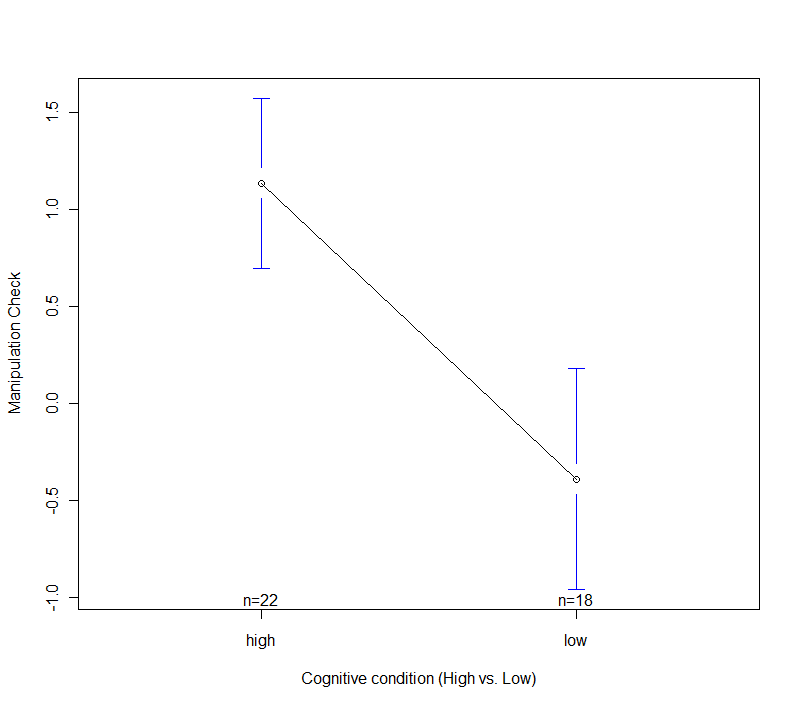
\includegraphics[width=7cm]{ManipulationCheck}
%    \caption{Average ratings for the manipulation check question}
%    \label{fig:ManipulationCheck}
%\end{figure}


Participants were asked in the post-questionnaire whether the video presented a
\emph{``robot kind of task''} or a \emph{``human kind of task''} on a 5-point
scale (numerical values ranging from -2 to 2, where -2 refers to robot kind of
task). We found a significant mean difference ($M_{\text{machine-like}}=TBD (SD=TBD)$
\vs $M_{\text{human-like}}=TBD (SD=TDB)$) in this
manipulation check ($F(1,54) = 29.0, p < .001$): the participants who watched
stimuli in the \emph{machine-like priming} condition identified the tasks as more
robot-like, while participants who watched the videos with a \emph{human-like
priming} perceived the tasks as more human-like.

Note that, expectedly, we found an order effect on the presentation of the robot
and human stimuli (our within-subject variable): if the stimuli shown last
involved a human, the participant reported a more human-like kind of tasks
(ANOVA between the models with condition only and condition and order: $F(1,51)
= 11.15, p < .001$, no interaction). This was accounted for by counter-balancing
the presentation order.

This first result supports \h{1}: cognitive priming enables us to
effectively elicit different levels of human-likeliness attribution.
\h{1} is however only partially supported as it specifically hypothesised that cognitive
priming can manipulate anthropomorphic attributions to the \emph{robot} itself:
the results of the manipulation check only indicate that the priming impacted
the participants' anthropomorphic perception of the \emph{interaction
situation} as a whole.

\subsection{Impact of Cognitive Priming on Anthropomorphic Attributions}

Running an ANOVA against the change of anthropomorphic attributions
\deltaant before and after the experiment shows that \deltaant is greater for the participants who watched the
human-like tasks ($\Delta_{\text{machine-like}}=TBD (SD=TBD)$
\vs $\Delta_{\text{human-like}}=TBD (SD=TDB)$, $F(1,54) = 6.54, p < .05$\fixme{put the exact
p value here}). In other words, after being exposed to short videos of a robot
performing simple tasks, participants primed with richer cognitive
expectations regarding the robot report a significantly higher tendency to anthropomorphise robots
\emph{in general} (as the questionnaire on anthropomorphic attributions
explicitly referred to \emph{robots in general}).

This result shows that the manipulation of the cognitive requirements of our
tasks does indeed alter the participants' perception of the robots themselves.
Combined with the previous result, we can conclude that \h{1} is indeed
supported: by the mean of cognitive priming, we can manipulate the
human-likeness attributions to robots.


%\begin{figure}
%    \centering
%    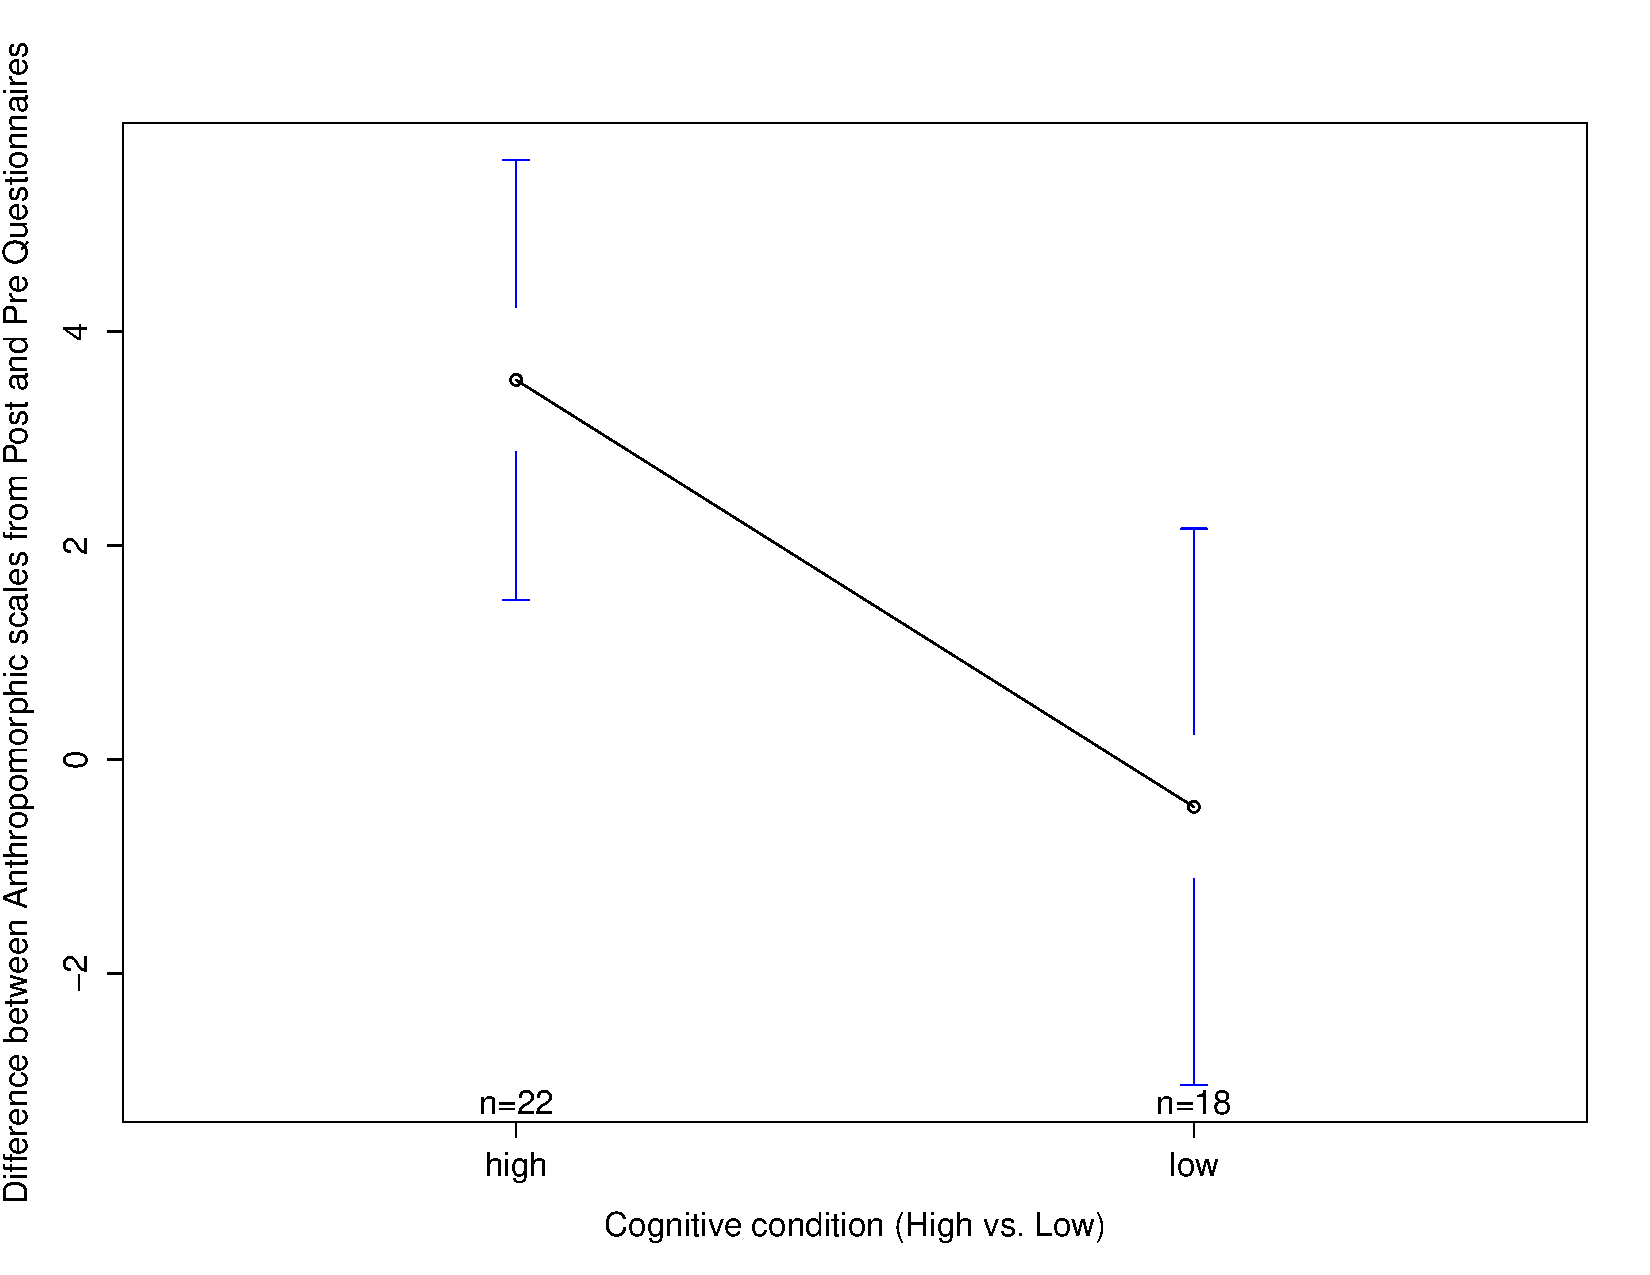
\includegraphics[width=3.3in]{H4}\label{ICAtoAAPImprovement}
%    \caption{Difference between \anti{} and \antf{} in the machine-like and
%    human-like
%    cognitive priming conditions.}
%    \label{h4}
%\end{figure}

This result also supports \h{4}: cognitive priming impacts the
attribution of anthropomorphic features to robots beyond the specific Nao robot
shown in the stimuli. It appears that participants transfer to some extent the
cognitive capabilities that they ascribe to the Nao robot in the
\emph{human-like} cognitive condition to robots in general. We can not, however,
conclude on any possible \emph{lasting} anthropomorphic ascriptions to robots as we
measure the anthropomorphic perception immediately after the experiment.


\subsection{Impact of the Tendency to Anthropomorphise on Human
Gazing Behaviours}

We found a significant negative correlation between
$\delta_{\mathcal{H},\mathcal{R}}^{\text{gaze}}$ and
the initial tendency to anthropomorphise \anti{} (Pearson Correlation Coefficient $r(54) = -0.43,
p < .001$, figure~\ref{h2}). The higher the (initial) tendency to anthropomorphise, the smaller
the difference in gazing behaviours between the robot and human conditions. This
supports hypothesis \h{2}.

\begin{figure}
    \centering
    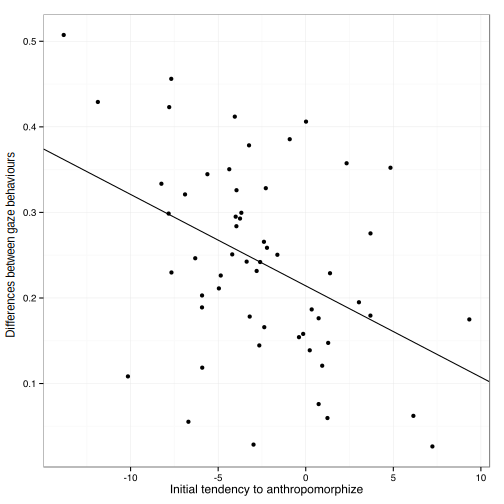
\includegraphics[width=0.5\columnwidth]{H2}\label{GazeDifference-vs-ICA}
    \caption{Gaze distribution difference $\delta_{\mathcal{H},
    \mathcal{R}}^{\text{gaze}}$ \vs initial tendency to anthropomorphise \anti{}}
    \label{h2}
\end{figure}

\subsection{Gaze Behaviours in Response to Machine-like \vs Human-like Cognitive Priming}

We consider the 5 groups of AOIs {\sf head}, {\sf arms}, {\sf hands}, {\sf
torso} and {\sf legs} (the left and right arms, hands and legs are grouped
together, other AOIs not belonging to the robot are left out). Based on ANOVA results for the robot in both the machine-like and human-like
cognitive priming conditions, the fixations on the head in the human-like condition
were found to be significantly higher than that in the machine-like condition
($F(1,54) = 4.2, p < .05$\fixme{put the exact p value here}). For all other AOIs groups, the fixations across
machine-like and human-like conditions were almost the same. Figure~\ref{h3} shows the
distribution of proportion of time spent gazing on the 5 AOI groups for the two
conditions.

\begin{figure}[ht!]
    \centering
    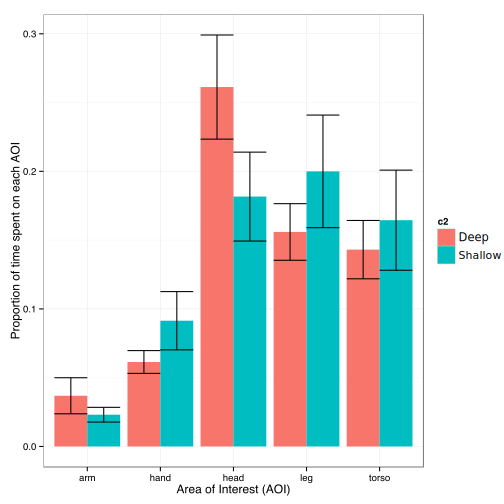
\includegraphics[width=0.6\columnwidth]{GazeHighLow}\label{GazeHighLow}
    \caption{Gaze fixations on the different areas on interest of the robot, for machine-like \vs
    human-like cognitive priming conditions. TBD: what do the error bar represent?}
    \label{h3}
\end{figure}

TBD: add plot human condition

This constitutes the main novel result of this study: priming an observer with
the expectation of a robot endowed with richer cognitive abilities leads to significantly longer
fixations on the robot's head, even though the actual behaviour of the robot is
the same (hypothesis \h{3}).

Note that we only analysed these possible correlations for robot condition: in
the human condition, the presence of the human is intrinsically a source of rich
cognitive expectations, masking the effects of our manipulation on a
machine-like \vs human-like cognitive priming.


%%%%%%%%%%%%%%%%%%%%%%

\section{Discussion}

The significant impact of the machine-like \vs human-like conditions on the
answers to the question \emph{Were the tasks more ``a robot kind of task'' or
``a human kind of task''?} shows that our manipulation was effective: framing
the interaction situation to induce a machine-like or a human-like task context
was successful. By further showing that the conditions also impact the
reported tendency to attribute anthropomorphic traits to robots in general (as assessed by
the Godspeed questionnaire), we conclude that our manipulation of the commands
given to the robot effectively influenced the participants in perceiving the
robot as anthropomorphic.

We interpret this result as the consequence of building in each condition a
different set of expectation regarding the cognitive skills of the robot: when a
participant hears the robot being instructed ``Pick up your favourite toy'', she
implicitly (and likely, unconsciously) supposes that the robot has the cognitive
capabilities required to \emph{prefer} one toy to another one, which would also
typically implies that the robot understand the affective dimensions of toys. By
performing this reasoning, the human would (likely unconsciously) attribute
cognitive and emotional traits to the robot that are akin to humans, and as a
result, anthropomorphise more the robot. Similarly for the command ``Point at
the crying baby'' that elicits not only emotional attributions related to cries
and babies, but also suggests that the robot has a sense of the urgency of
the situation (a baby is crying!). Our manipulation makes the robot appear as it
possesses a commonsense knowledge of a typically human situation.

Remarkably (and in line with the literature reviewed in
section~\ref{cognitive-priming}), these cognitive ascriptions lead to a visible
change in the participants' behaviour: they gaze more at the head of the robot
when they watch a scene that elicits stronger anthropomorphic attributions.
Several explanations can be thought of. At an abstract level, the head may
typically be seen as embodying the mind and the emotions. As such, the head of
an agent that is believed to be endowed with such cognitive and emotional
abilities could be thought to be of higher importance, attracting more
attention. Another explanation pertains to the social norms elicited by a moral
agent~\citep{malle2014moral}. We can reasonably suppose that a robot thought to
be endowed with rich cognitive skills is likely to be considered more as a moral
agent as a robot with an apparent mechanical behaviour. As a result, the
participant might be led to adhere to social norms (including looking at the
face when interacting) when watching the robot. A third explanation involves
automatic social behaviours: if the participant is tricked into believing that
the robot might have a richer set of cognitive skills, she might automatically
search for other socio-cognitive confirmation cues, and the face is a
particularly rich source of such cues (facial expressions, gaze, back-channel
communication like nodding). This would therefore also lead to longer observed
gaze fixations on the robot's head.

Our experimental protocol enabled us to examine two additional questions: by
administrating the Godspeed questionnaire on anthropomorphism and mind
attribution first as pre-test, we gained a picture of the initial tendency of
our participants to anthropomorphise robots. Using our \deltaant measure of the
gazing behaviour similarity, we have evidenced that people with an higher
tendency to anthropomorphise robots, also exhibit a more similar gazing
behaviour when they watch either a human or a robot performing the same task. If
confirmed (in particular with balanced human genders), this is a significant
result. The Godspeed questionnaire assesses how likely we are to
anthropomorphise machines in an abstract way: no concrete robots nor interaction
situations are shown; the participants might react to the sentence ``Please rate
your impression of robots'' in widely different ways depending on their own
constructed images of what robots are. And yet, our results show a significant
correlation with gazing behaviour: the more you tend to anthropomorphise, the
more you look at robots the way you look at humans. This implies that the mere
propensity to attribute physical or mental human traits to robots suffice to
influence a mostly unconscious (yet easy to observe) physical behaviour.  This
link between psychological attributions and a resulting physical behaviour might
be of interest to the Human-Robot Interaction community, especially if we endow
the robot with the ability to measure itself, \emph{during} the interaction, the
time spent by the human on its face. This would for instance allow the robot to
build an initial model of the cognitive expectations held by the human regarding
the robot.



Hypothesis \h{2} looked at a possible interaction between our tendency to
anthropomorphise (as measured in the pre-questionnaire) and our actual gaze
behaviour, the hypothesis being that high anthropomorphisers would show smaller
differences between the way they look at robots and humans (since they would
consider robots closer to humans than low anthropomorphisers). Our data supports
this hypothesis: participants reporting an higher tendency to anthropomorphise
tend to have closer gazing behaviours when they look at humans or at robots:
statistically speaking, the tendency to anthropomorphise robots
is reflected in the way one looks at them: you look at them
like you would look at humans.

The third hypothesis \h{3} proposes that head fixations are related to the
cognitive expectations, which is clearly supported by our data: after human-like cognitive
priming, one tends to spend more time looking at the head of the interacting
agent than after machine-like cognitive priming. We also hypothesised that, in turn,
head fixations could act as a \emph{proxy to anthropomorphic projections}: as
underlined in the previous section, our data also support this.

Finally, the hypothesis \h{4} looks at the dynamic of anthropomorphic
projections, with the hypothesis that watching an interaction with a particular
robot after a human-like cognitive priming may impact \emph{globally} the
anthropomorphic perceptions of robots. This is supported by our study.

\paragraph{Design of the Stimuli and Applicability of the Method to Real World
Scenarios}
\label{stimuli_design}

The video stimuli had to obey to several constraints: they had to depict
plausible and legible situations, yet simple enough to be suitable for an
eye-tracking study (simple mechanics, easily distinguishable elements at
predictable locations). The body parts of the robot or human would need remain
visible most of the time. The actions had to be meaningful for both a robot and
a human, and both should be able to perform them in similar ways (similar pace,
similar movements) without looking awkward.

Finally, the situations needed to support two possible kind of cognitive priming
(machine-like \vs human-like cognitive priming), and triggering one or the other of these
contexts needed to be done \emph{without changing} the visual part of the
stimulus.

We initially prepared three different stimuli: the \emph{Picking} task, the
\emph{Pointing} task and a \emph{Dance} task.  During the \emph{Dance} task, the
agent was either asked to \emph{``Show some movements''} (\emph{machine-like
cognitive priming} condition) or to \emph{``Dance with the music''}
(\emph{human-like cognitive priming} condition). While all the participants were
shown this stimuli as well, we decided to exclude it from the results as we
found out that the nature of the task (participants had to watch body movements)
introduced an experimental bias: because dance is a form of whole-body
expression, gazes where evenly distributed on the body of the agents, masking
possible cognition-related gaze patterns.

This underlines the difficulty of designing appropriate stimuli and raises the
question of the applicability of our method to real-world, ``in the wild''
human-robot interaction.

Two main comments can be made: first, we had to carefully design those stimuli
to \emph{evidence} the link between the (anthropomorphic) perception of a robot
and actual gaze fixations on the face of the robot. This being granted,
researchers will not have to design their scenarios in such a constraint way to
rely on our result, \ie the link between perception and gaze behaviour.

Besides, one may point that, in real-world experiments, the robot does not
always remain in the field of view of the participant, and, at the very least, the
body of the robot may be partially occluded at time.  This is certainly true,
and while new experiments would be welcome to validate it, we believe that our
method remains effective in these situations. First it relies on the
\emph{ratio} of the gaze fixations on the head \vs gaze fixations on other parts
of the body, thus compensating for out-of-sight robots; second, our method
\emph{does not} provide an \emph{absolute} measurement of the level
anthropomorphic perception, but rather a \emph{relative} measurement: within a
group of participants, it enables to classify participants in term of their level of
projected anthropomorphism onto the robot.  This means that, while this method
can not be used to assess the perception of robots between different interaction
situations (\ie different experiments), it can be employed within a group a
participants taking part to the same experiment.

Lastly, the stationary eye-tracker would also have to be replaced by a mobile
eye-tracker. This would however not impact the interpretation of the results.

\section{Conclusion}
\label{conclusion}

The study and results presented in this article lead to two main contributions:
new insights on the impact of the cognitive priming on the perception of a robot
by humans; a novel unbiased methodology based on eye-tracking to assess
anthropomorphic attributions during a running human-robot interaction.

Our first contribution extends our understanding of the attribution of
human-like characteristics to robot by exploring the role of the interaction
context. As we show, it appears that even relatively subtle context
priming may lead to significantly different anthropomorphic perceptions of
the exact same robot, performing the exact same task, as confirmed both by
distinct gaze patterns, and different reported perceptions in questionnaires.
Interestingly, this effects can already be evidenced after very short,
one-way, interactions (less than 2 minutes).

This leads to a second-order effect that we also evidence here: depending on the
cognitive priming, the tendency to attribute human-like characteristics to robot
evolves in significantly different ways. After observing a robot in a
context that presupposes richer cognitive capabilities, people increase
their general tendency to anthropomorphise robots compared to a machine-like
cognitive priming, even though the robot appearance and visual behaviour is the
exact same.

The second contribution is a methodological one: we present in this article
a novel technique to assess anthropomorphic projections that relies on a
biometric measure (eye-tracking) to compare gaze fixation durations on
the face of the robot. We cross-validate this new metric with existing,
established, questionnaires. Compared to current techniques (post-hoc
annotations of videos and questionnaires), this new approach is objective,
is less impacted by experimental biases (like the \emph{observer effect},
where the behaviour of the participant is impacted by the fact he/she knows that
he/she is observed) and take place during the interaction itself
(\emph{in-the-moment} measurement).

Besides, we also introduce a new kind of visual stimuli, specifically designed
to study the impact of non-appearance, non-behavioural related effects on the
human-like perception of robots. We make these video stimuli available to the
community, and therefore invite our colleagues to reproduce our experimental
results. The next section describe the specificities of these stimuli, and also
discuss how such a methodology can apply to real-world scenarios.

As a whole, the article attempts to contribute to our understanding of an
intricate psychological effects that come to play when humans and robots
interact, both in terms of methodology and experimental evidence.

\fixme{Properly conclude the paper: what does our research reveals?}

\section*{Acknowledgments}

We would like here to acknowledge the contribution of Julia Fink to a better
understanding of anthropomorphism as a psychological phenomenon. We also thank
all the students for their participation.

This research was supported by the Swiss National Science Foundation through the
National Centre of Competence in Research Robotics.

\newpage


\section {To be discussed}


% new results up for discussion on Skype
\subsection{Manipulation check - H1}


\begin{table}[ht]
\caption{Ordinal linear regression table for the manipulation check vs. cognitive context.}
\centering
\begin{tabular}{rrrrr}
  \hline
 & Value & Std. Error & t value & p value \\ 
  \hline
cond low & -2.52 & 0.57 & -4.39 & 0.00 \\ 
  -2$|$-1 & -4.06 & 0.66 & -6.19 & 0.00 \\ 
  -1$|$0 & -2.17 & 0.48 & -4.57 & 0.00 \\ 
  0$|$1 & -1.24 & 0.40 & -3.08 & 0.00 \\ 
  1$|$2 & 0.05 & 0.35 & 0.15 & 0.88 \\ 
   \hline
\end{tabular}
\end{table}



\subsection{Gaze difference vs. \anti levels- H2}



\begin{table}[ht]
\caption{\anti levels - high, low, neutral}
\centering
\begin{tabular}{rrrrr}
  \hline
 & diff & lwr & upr & p adj \\ 
  \hline
l-h & 0.10 & 0.02 & 0.18 & 0.01 \\ 
  n-h & 0.03 & -0.10 & 0.17 & 0.80 \\ 
  n-l & -0.06 & -0.18 & 0.06 & 0.44 \\ 
   \hline
\end{tabular}
\end{table}


\subsection{H3- the results remain the same}

One more result in deep (high) cognitive condition the participant stay on the head for longer periods, 

We had a comment from the reviewers: `` In addition, you need to address that
head fixations to the robot could increase because people are curious whether
the robot really has the implied capacities, not because they assume it has
them. Can you rule out this alternative interpretation?'' 

they leave other parts of body earlier and leave the head later this might reflect a hypothesis verification by the participants

\begin{table}[ht]
\caption{transition to and from ``head'' and Duration of looking at head}
\centering
\begin{tabular}{rrr}
  \hline
 & to & from \\ 
  \hline
high & 1441.075(-3.31) & 2646.870(2.62) \\ 
  low & 1882.956(3.14) & 2670.569(-2.48) \\ 
   \hline
\end{tabular}
\end{table}




MORE TO APPEAR``reported eye tracking results are far too cursory'' - I will put
a nice factor analysis of the eye-tracking data with the questionnaire responses
and then we can answer many questions in the results section. 

\bibliographystyle{apacite}
\bibliography{biblio}

\pagebreak
\appendix

\section{Appendices}

The video stimuli, questionnaires results, eye-tracking data and R scripts for
the analysis are all available at
\url{https://github.com/chili-epfl/anthropomorphism-eyetracking}.

The pre- and post-questionnaires are reproduced hereafter.
\vfill
\pagebreak
\paragraph{Pre-questionnaire} (2 pages)

\begin{center}
    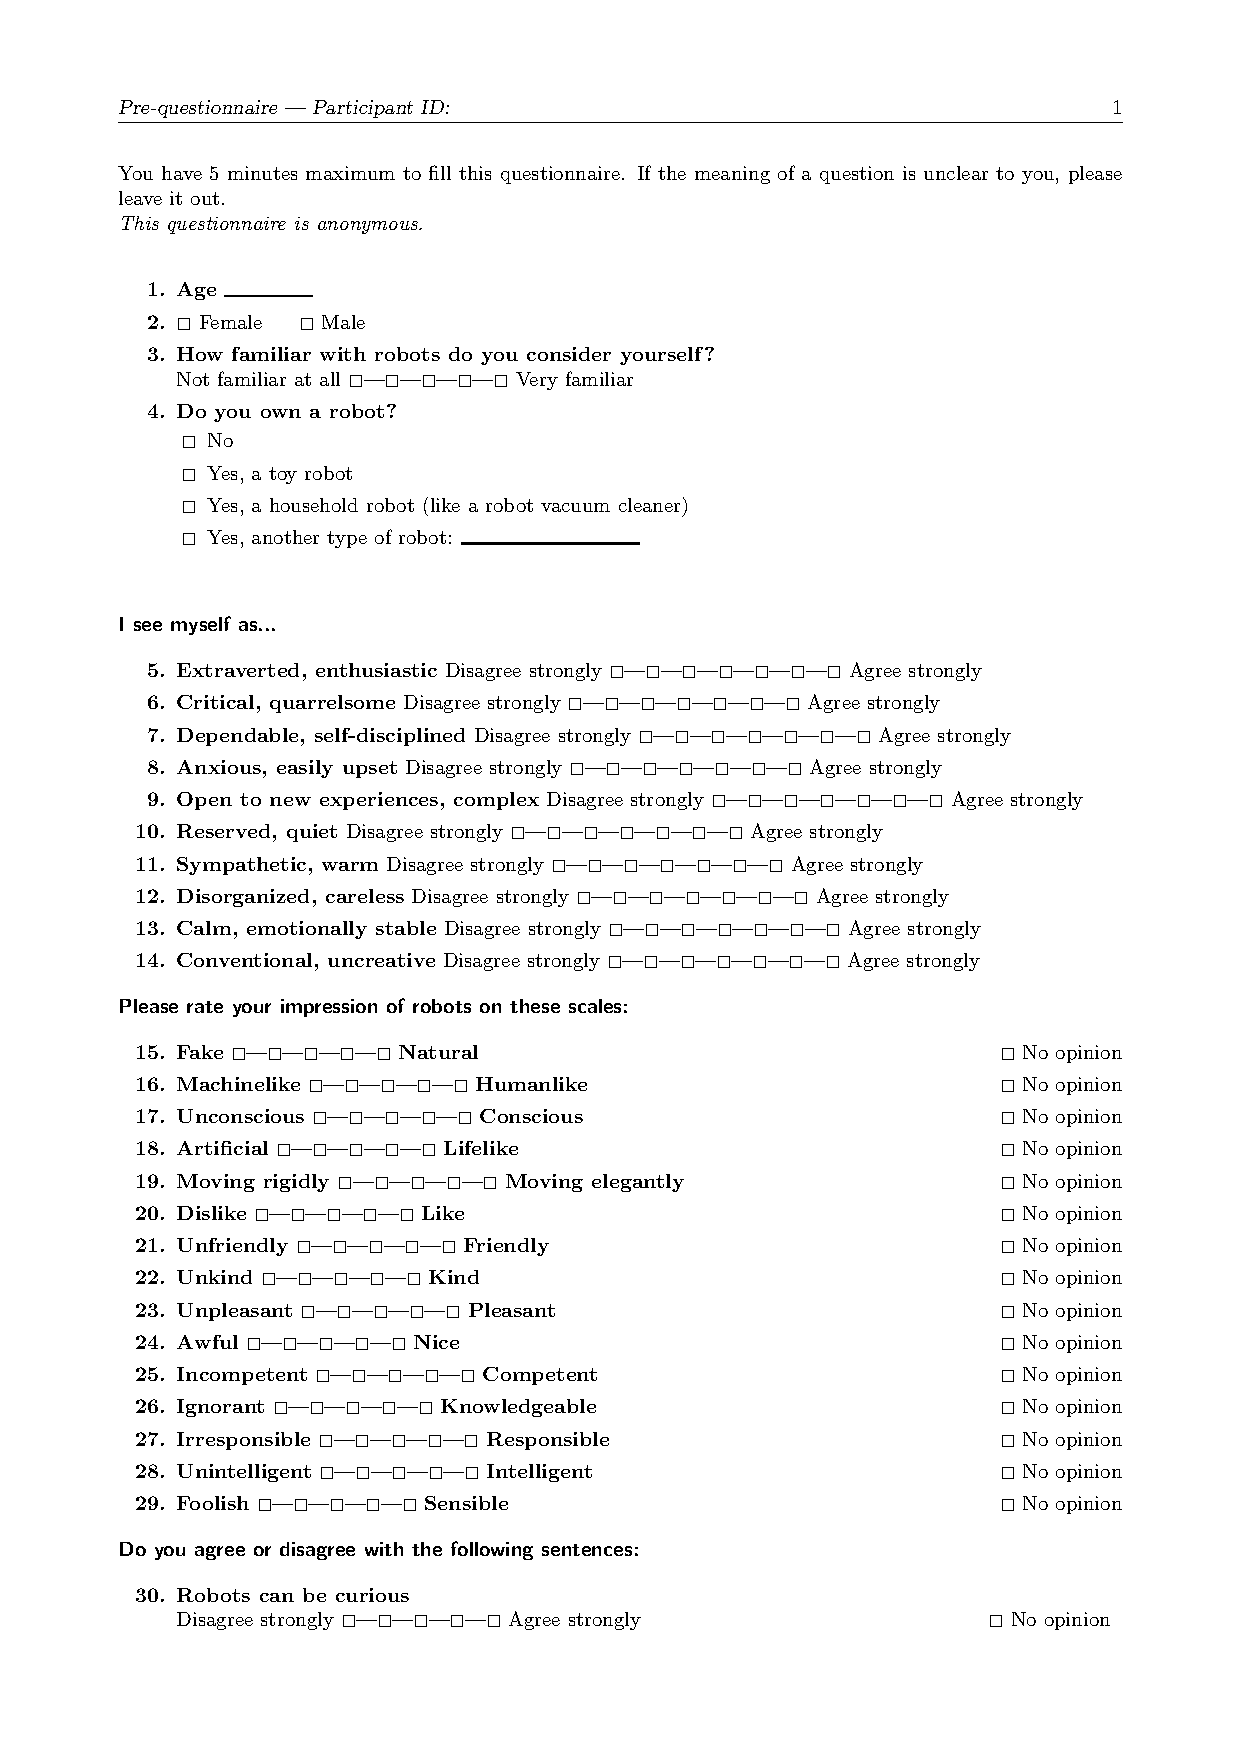
\includegraphics[width=0.9\linewidth]{pre-questionnaire}

    \includegraphics[width=0.9\linewidth, page=2]{pre-questionnaire}
\end{center}

\pagebreak
\paragraph{Post-questionnaire} (2 pages)

\begin{center}
    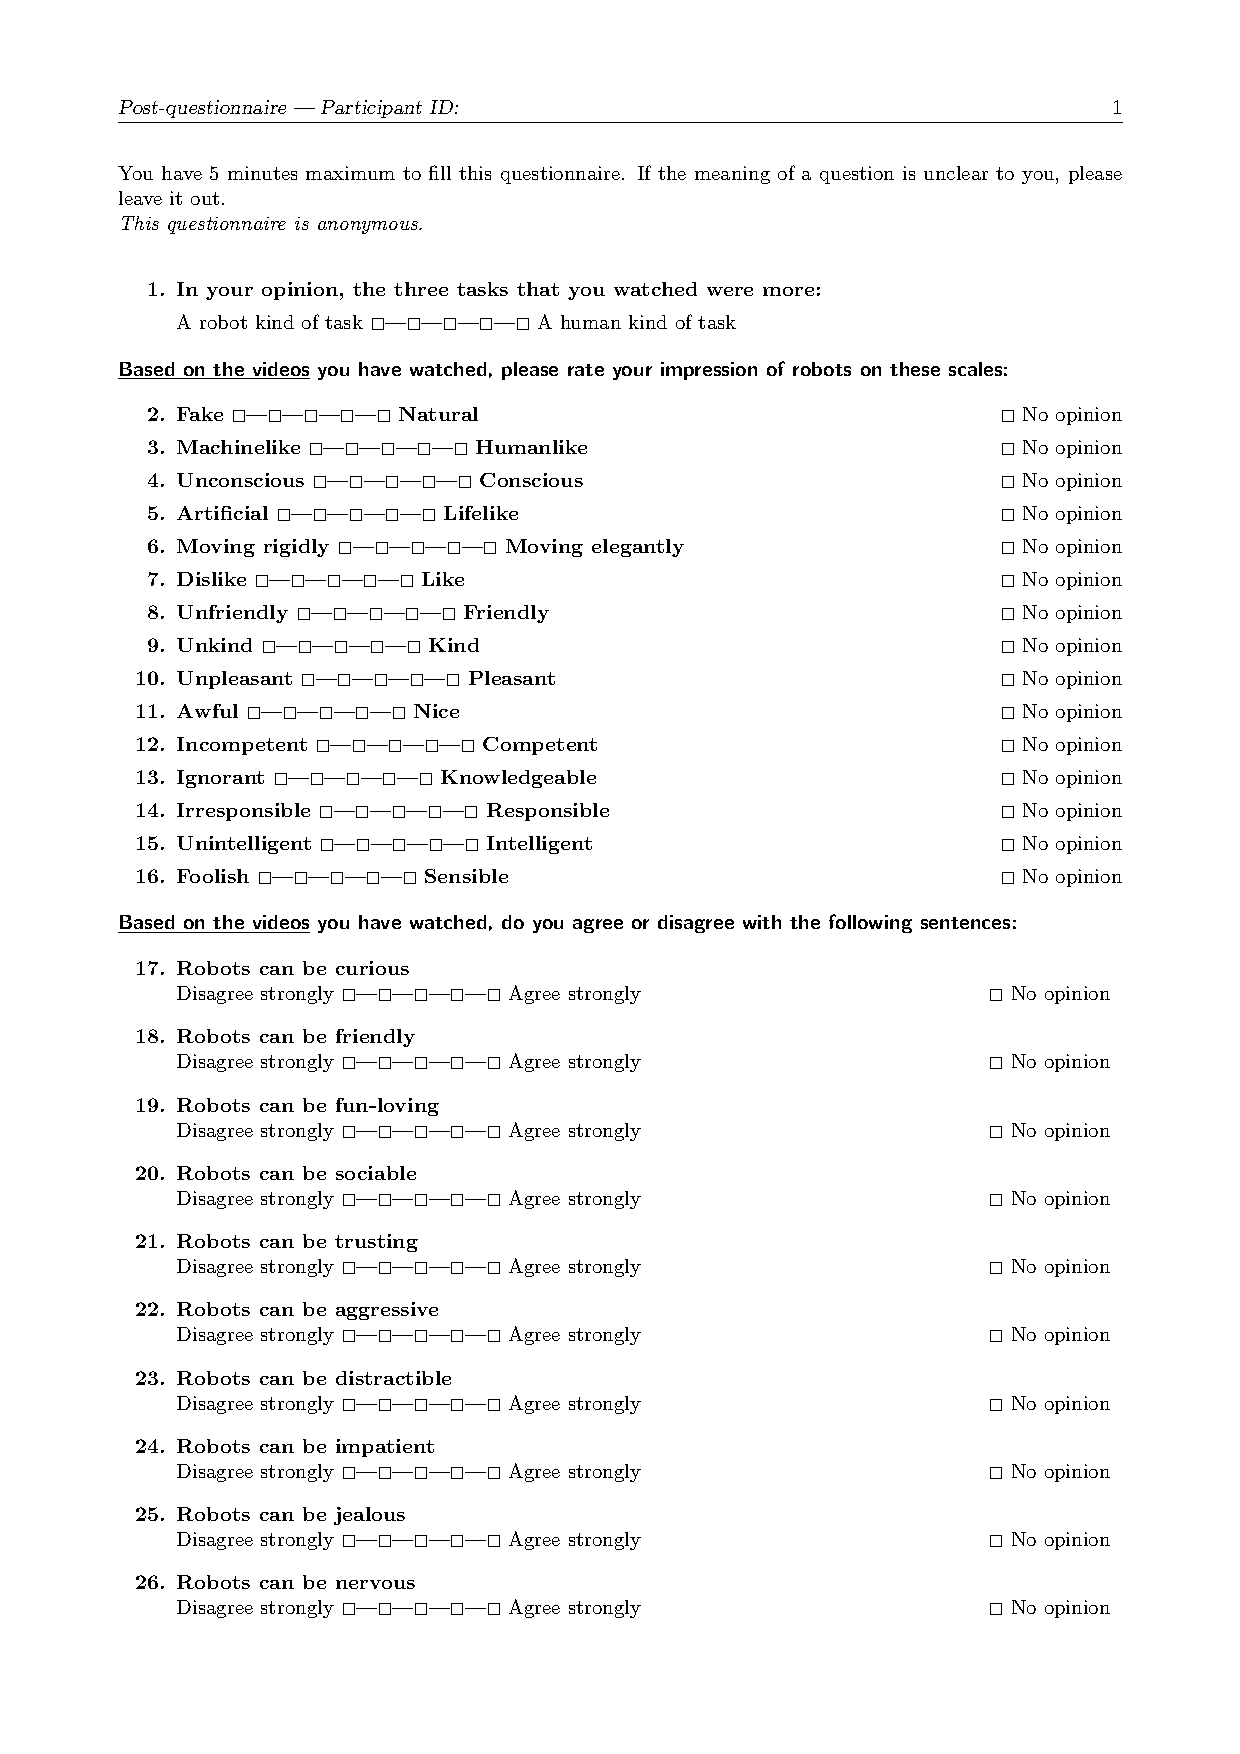
\includegraphics[width=0.9\linewidth]{post-questionnaire}

    \includegraphics[width=0.9\linewidth, page=2]{post-questionnaire}
\end{center}
%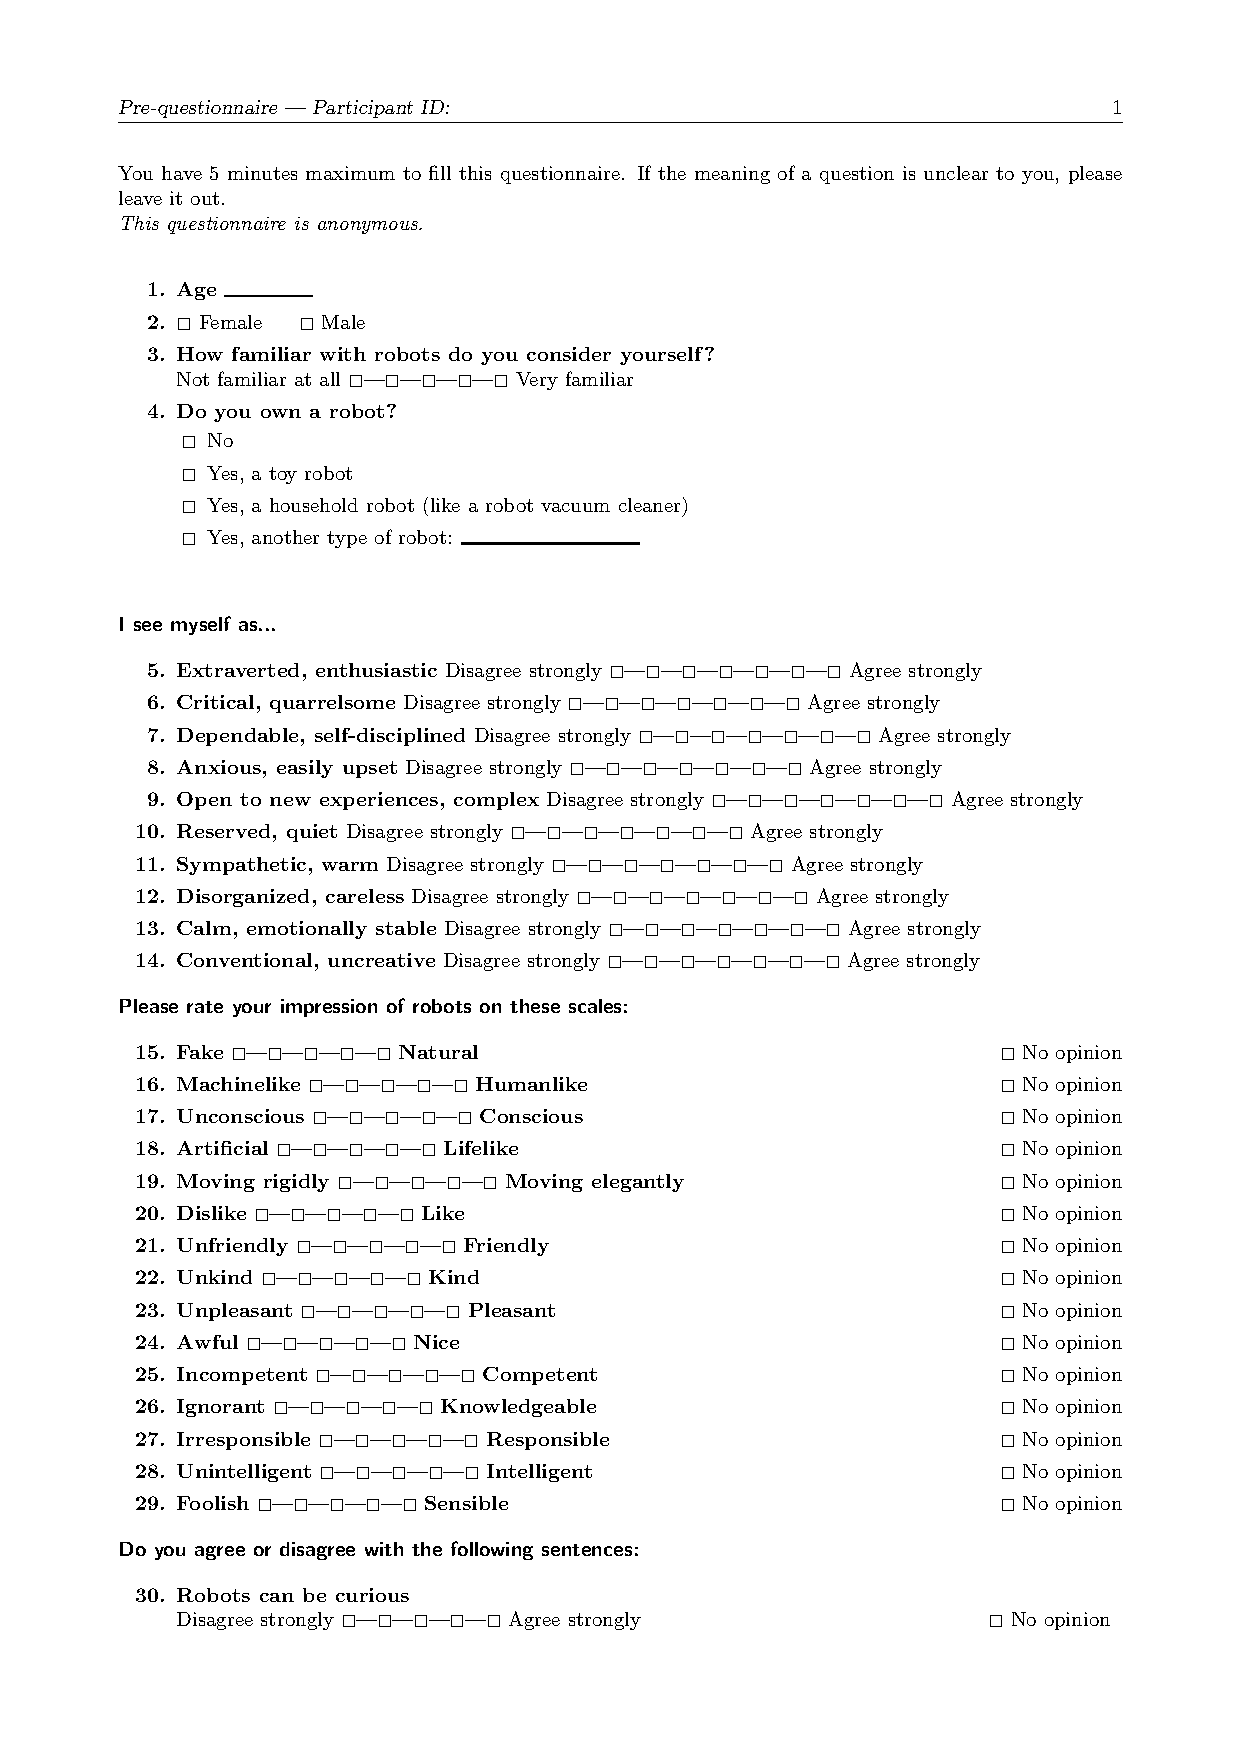
\includepdf[pages={1,2}]{pre-questionnaire.pdf}
%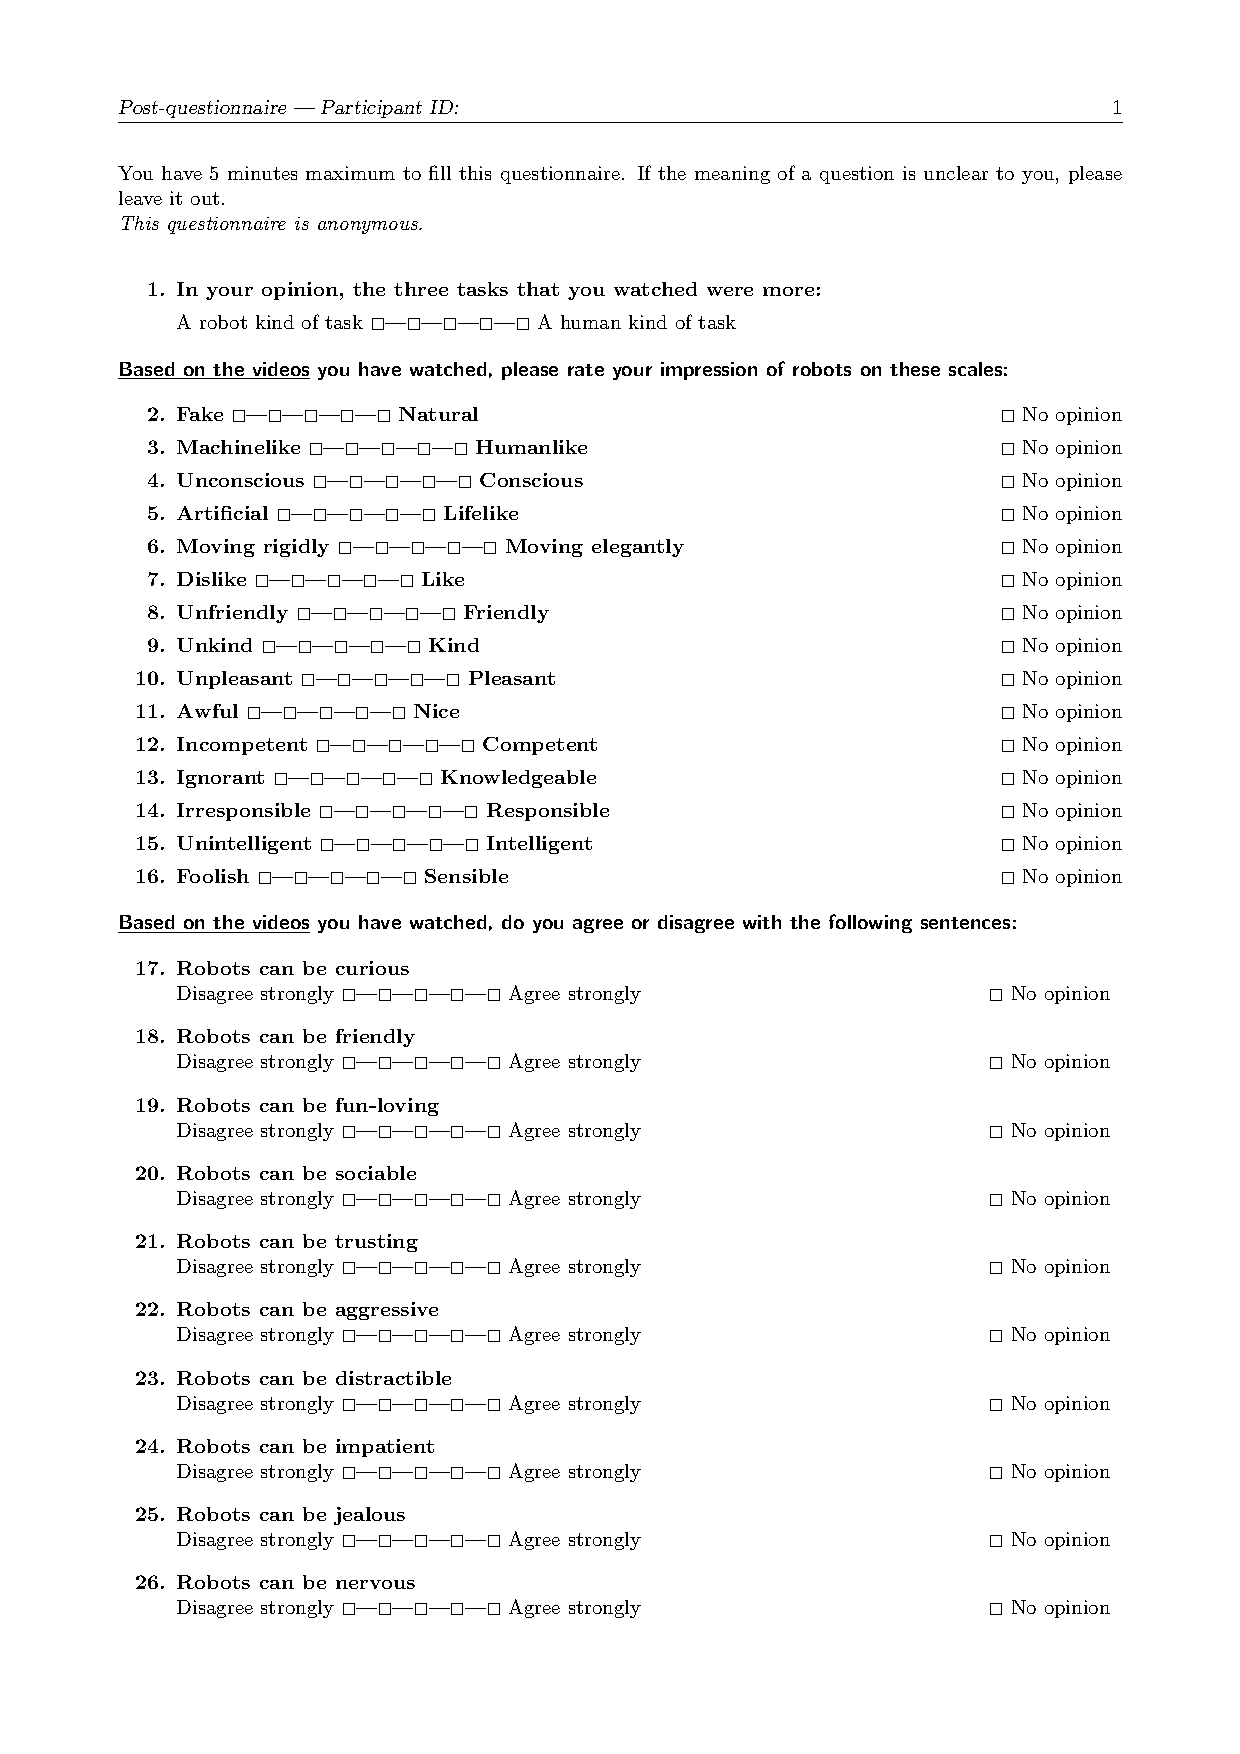
\includepdf[pages={1,2}]{post-questionnaire.pdf}

\end{document}
